\documentclass{article}
\usepackage[utf8x]{inputenc}
\usepackage[english,russian]{babel}
\usepackage{graphicx}
\usepackage{todonotes}
\usepackage{hyperref}
\begin{document}
\title{Применение формулы Кирхгофа для задачи миграции}
\author{\textbf{Голубев В.И.} \\ Лаборатория прикладной вычислительной геофизики МФТИ}
\maketitle
Согласно выводу (уравнени 15.208), приведённому в книге Жданова, распределение давления для
задачи акустики, показывающее также и положение отражающих границ,
может быть найдено на основе формулы Рэлея для случая горизонтальной плоскости
наблюдения:
\begin{equation}
\label{rayleigh_migration}
U^m(\vec{r'},0) = -\frac{1}{2\pi}\frac{\partial}{\partial z'}
	\int_S \frac{U(\vec{r},\frac{2|\vec{r'}-\vec{r}|}{c})}{|\vec{r'}-\vec{r}|}ds,
\end{equation}
где $U$ - скалярное поле давления, $\vec{r}$ - координата на поверхности, в которой записывается
сейсмограмма, $\vec{r'}$ - координата в объёме, где ищется мигрированное изображение, $c$ - скорость распространения возмущения, стоящая в волновом уравнении (уравнение 13.54):
\begin{equation}
\label{wave_equation}
\nabla^2P(\vec{r},t) - \frac{1}{c^2(\vec{r})}\frac{\partial^2}{\partial t^2}
	P(\vec{r},t) = - F^e(\vec{r},t).
\end{equation}

\section{Изображение точечного источника}

Рассмотрим пример генерации синтетической сейсмограммы $U(\vec{r}, t)$ точечным источником, расположенным в однородной среде в точке $\vec{r_o}$.
Согласно формуле (13.72) решение в данном случае имеет вид (момент действия источника $t = 0$):
\begin{equation}
\label{point_source}
U(\vec{r}, t) = \frac{1}{4\pi|\vec{r} - \vec{r_o}|}\delta(t - \frac{|\vec{r} - \vec{r_o}}{c}).
\end{equation}

Подставляя формулу (\ref{point_source}) в формулул (\ref{rayleigh_migration}) получим:
\begin{equation}
\label{point_source_migrated}
U^m(\vec{r'}) = -\frac{1}{8\pi^2}\frac{\partial}{\partial z'}\int_S \delta(\frac{2|\vec{r'} - \vec{r}| - |\vec{r} - \vec{r_o}|}{c})\frac{ds}{|\vec{r} - \vec{r_o}||\vec{r'} - \vec{r}|}.
\end{equation}

Выражение может быть приобразовано к виду:
\begin{equation}
\label{point_source_migrated_xy}
U^m(x',y',z') = -\frac{1}{8\pi^2}\frac{\partial}{\partial z'} \int\limits_{-\infty}^{\infty} \int\limits_{-\infty}^{\infty} \frac{\delta(\frac{2\sqrt{(x-x')^2 + (y-y')^2 + z'^2} - \sqrt{(x-x_0)^2 + (y-y_0)^2 + z_0^2}}{c})dxdy}{\sqrt{(x-x')^2 + (y-y')^2 + z'^2}\sqrt{(x-x_0)^2 + (y-y_0)^2 + z_0^2}}.
\end{equation}

Необходимо отметить, что не очевидно, что выражение (\ref{point_source_migrated_xy}) будет иметь особенность в точке источника.
Был проведён тестовый расчёт компьютерной программы (см. следующий раздел) на точечном (по пространству) источнике.
Временная функция источника - Ricker wavelet с частотой 50 Гц.
На странице \url{http://utam.gg.utah.edu/UTAMtheses/HongchuanSun/html/node13.html} удалось найти пример с параметрами модели и результатом миграции Кирхгофа.
Кстати, по-видимому, там опечатка и скорость среды 2500 м/с, а не 5000 м/с, т.к. иначе их сейсмограмма не верная!
На рис. \ref{comparison_1} представлено изображение, полученное после процедуры миграции с теми же самыми параметрами среды и источника и расчётной сетки.
\begin{figure}[ht]
  \center
  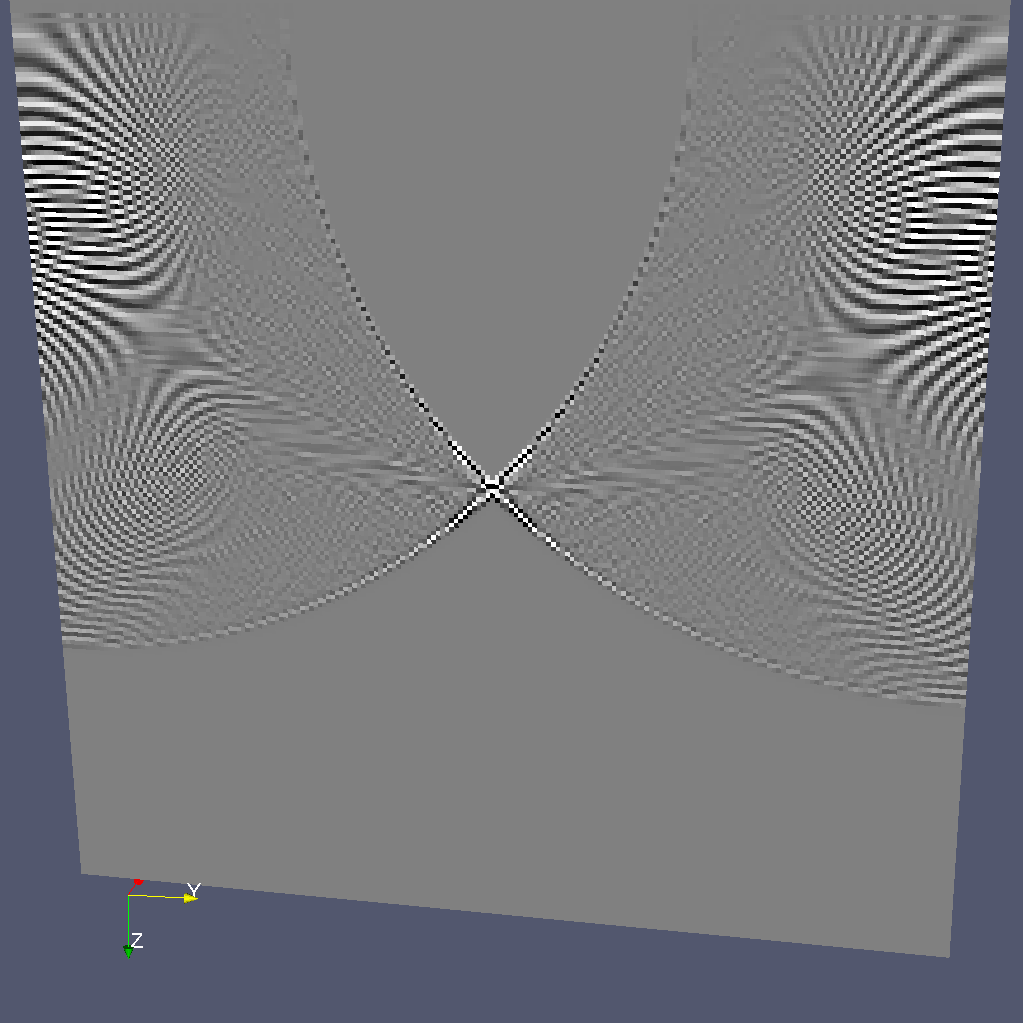
\includegraphics[scale=0.2]{pic/point_source_2000_2000.png}
  \caption{Мигрированное изображение. Источник точечный (Ricker 50 Hz), находится в точке 2000, 2000 (ноль в верхнем левом углу).}
\label{comparison_1}
\end{figure}

Также дополнительно был проделан расчёт с изменением положения источника. На рис. \ref{comparison_2} источник располагался в точке 3000, 700.
\begin{figure}[ht]
  \center
  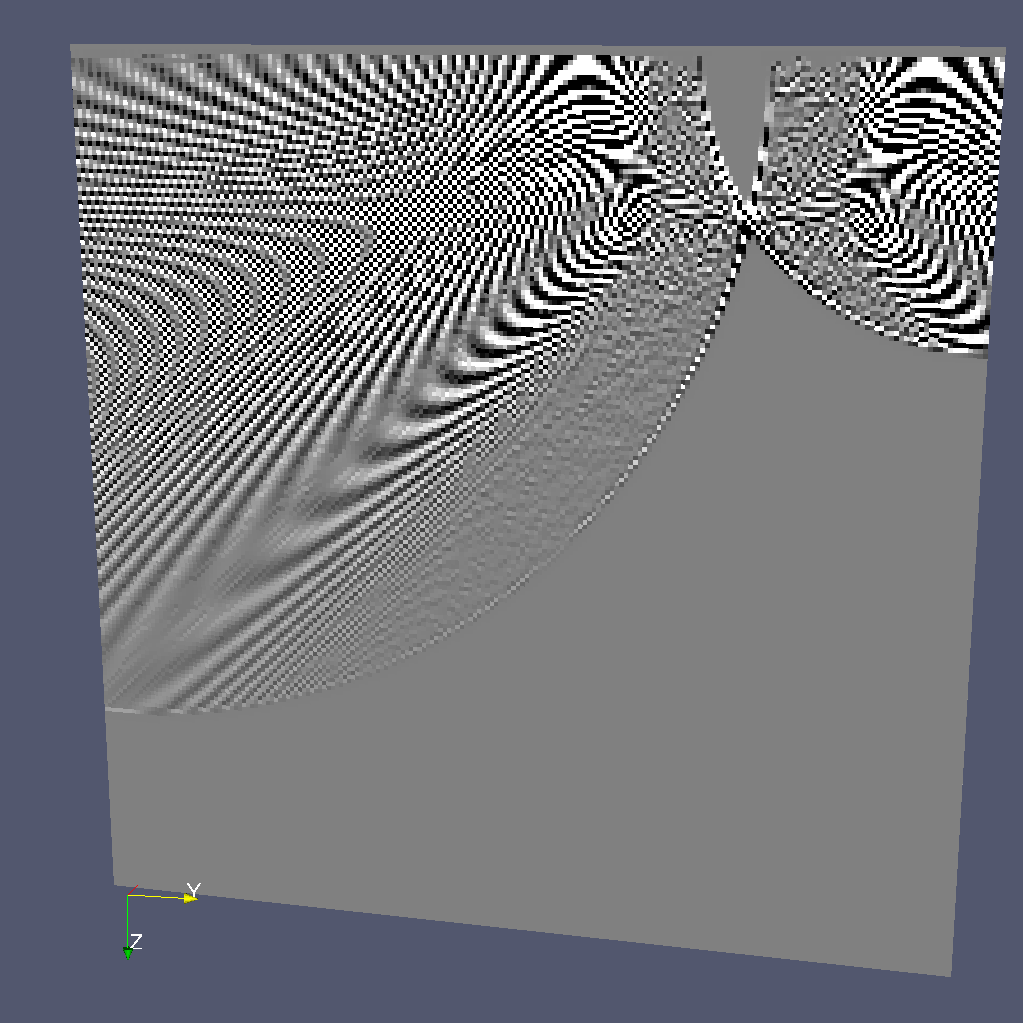
\includegraphics[scale=0.2]{pic/point_source_3000_700.png}
  \caption{Мигрированное изображение. Источник точечный (Ricker 50 Hz), находится в точке 3000, 700 (ноль в верхнем левом углу).}
\label{comparison_2}
\end{figure}

Хорошо видно, что мигрированное изображение отображает положение источника.
Кстати, чтобы не возникало сомнений по поводу сравнения с примером в Интернете в плане интенсивности привожу в другой шкале при отображении (так, что границы теперь больше по модулю, чем были).
\begin{figure}[ht]
  \center
  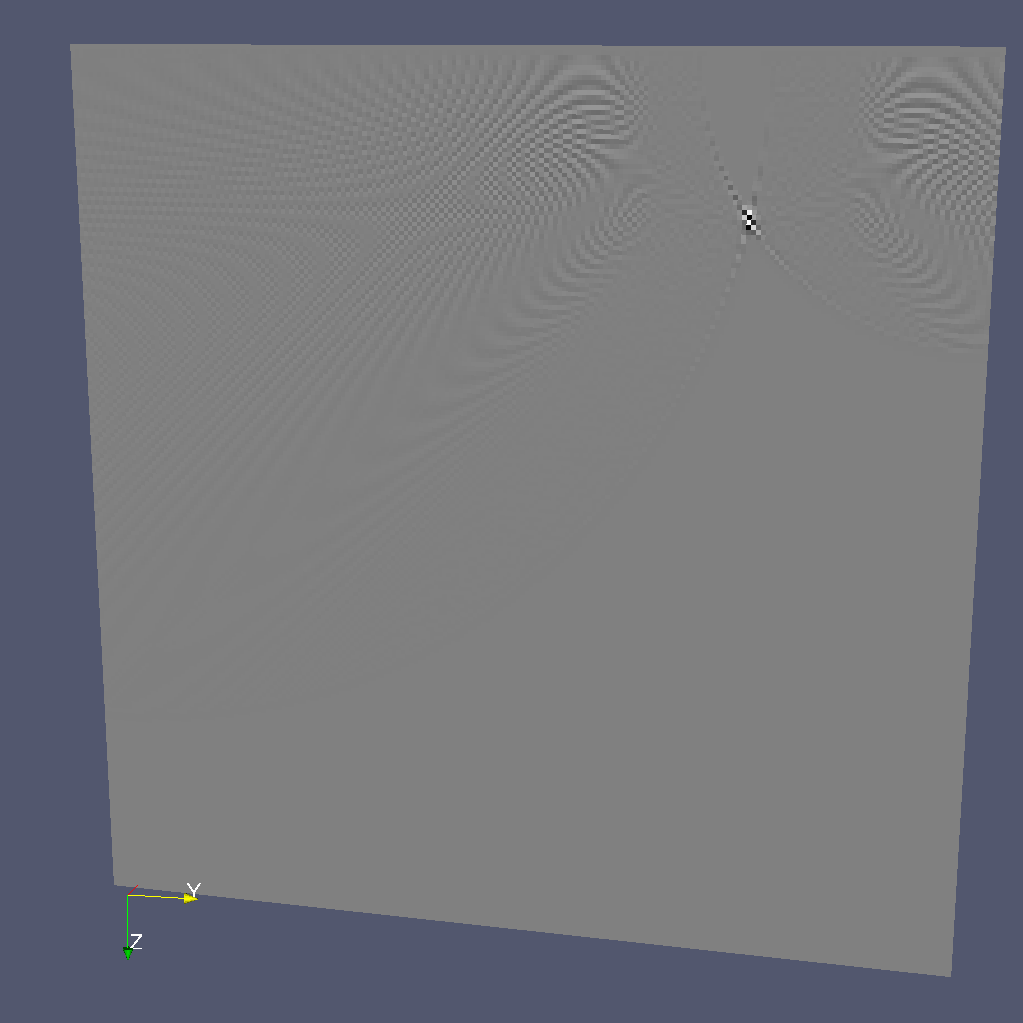
\includegraphics[scale=0.2]{pic/point_source_3000_700_val.png}
  \caption{Мигрированное изображение. Источник точечный (Ricker 50 Hz), находится в точке 3000, 700 (ноль в верхнем левом углу). Изменил пределы отрисовки и видно, что шумы по бока обладают значительно меньшей интенсивностью}
\label{comparison_3}
\end{figure}

\section{Численная реализация}

Рассмотрим простейший случай, когда расчётная сетка кубическая, и на поверхности сейсмоприёмники расположены в каждом её узле.
В таком случае формула (\ref{rayleigh_migration}) может быть записана в виде:
\begin{equation}
\label{rayleigh_migration_discrete}
U^m(i,j,k) = -\frac{1}{2\pi}\frac{\sum\limits_{l,m} \frac{U(l,m,\frac{2d(i,j,k+1,l,m)}{c})}{d(i,j,k+1,l,m)}\delta x \delta y - \sum\limits_{l,m} \frac{U(l,m,\frac{2d(i,j,k,l,m)}{c})}{d(i,j,k,l,m)}\delta x \delta y}{\delta z},
\end{equation}
где $d(i,j,k,l,m)=\sqrt{(l-i)^2(\delta x)^2 + (m-j)^2(\delta y)^2  + (k)^2(\delta z)^2}$, а начало координат находится в точке $(i,j,k)=(0,0,0)$.
В дальнейшем может быть проведено обобщение на случай произвольной (на дневной поверхности!) расстановки приёмников.

Был реализован прототип вычислителя, работающего по описанному алгоритму.
Для простоты не проводилось никакой интерполяции ни во временной области, ни в пространственной области для сейсмограмм, а просто брались значения из ближайшего пространственно-временного отсчёта.
Выполнено тестирование на двух задачах миграции.
\todo[inline]{ДАЛЬШЕ В ТЕСТАХ ИСПОЛЬЗОВАЛ НЕ ТОЧЕЧНЫЙ ИСТОЧНИК, НЕВЕРНО!!!}
В первом случае задавалась синтетическая сейсмограмма, полученная при отклике, инициированном продольной вертикально падающей волной с шириной фронта 400 м, от границы раздела, расположенной на глубине 1000 м.
Во втором случае граница раздела у $\frac{1}{3}$ области по горизонтали (считая от начала координат) находилась на глубине 500 м, у $\frac{2}{3}$ - на глубине 1000 м.
Вся расчётная область составляет 1500 м.
На рис. \ref{layers_inverted} представлено изображение, полученное после процедуры миграции.
\begin{figure}[ht]
  \center
  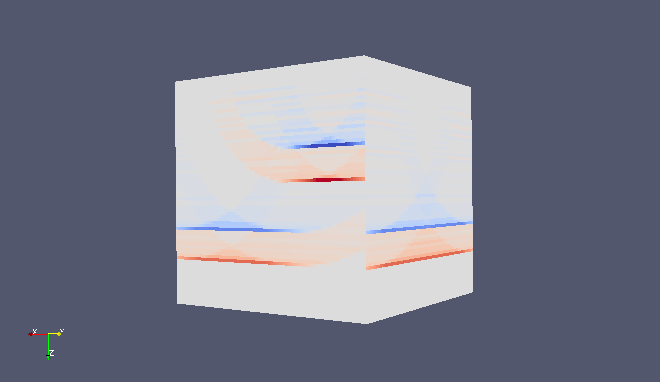
\includegraphics[scale=0.5]{pic/layers_inverted.png}
  \caption{Мигрированное изображение (слева - разрывная граница, справа - сплошная). Синий цвет - отрицательные значения, красный - положительные.}
\label{layers_inverted}
\end{figure}
\end{document}
